\documentclass{article}
\usepackage{tikz}
\usetikzlibrary{arrows.meta,positioning,shapes.geometric}
\usepackage{pgfplots}
\pgfplotsset{compat=1.18}
\begin{document}
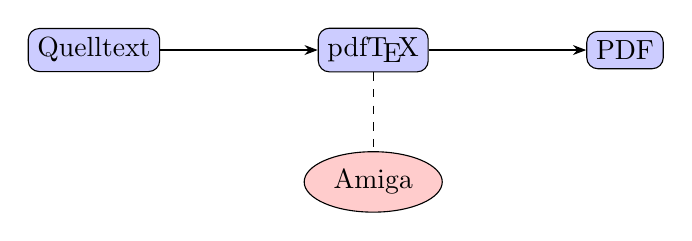
\begin{tikzpicture}[node distance=2cm,box/.style={draw,rounded corners,fill=blue!20}]
\node[box](a){Quelltext};\node[box,right=of a](b){pdf\TeX};\node[box,right=of b](c){PDF};
\draw[-{Stealth}](a)--(b);\draw[-{Stealth}](b)--(c);
\node[draw,ellipse,below=1cm of b,fill=red!20](d){Amiga};\draw[dashed](b)--(d);
\end{tikzpicture}

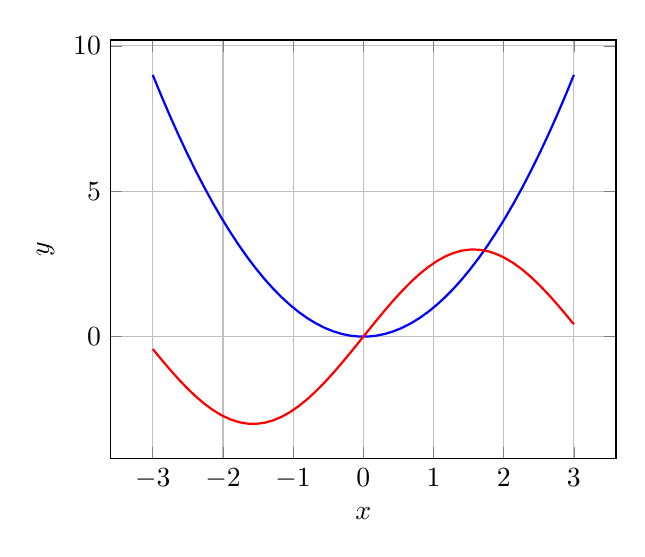
\begin{tikzpicture}
\begin{axis}[xlabel=$x$,ylabel=$y$,grid=major,width=8cm]
\addplot[blue,thick,domain=-3:3,samples=50]{x^2};
\addplot[red,thick,domain=-3:3,samples=50]{sin(deg(x))*3};
\end{axis}
\end{tikzpicture}
\end{document}
